%!TEX root = ../Main.tex

\chapter{implementation}

\subsection{Overview}
To give an overview of the software for the system a class diagram have been made. This can be seen on the figure below.
On class diagram have been developed based on the former domain problem analysis such as use cases. When a somewhat sufficient class diagram had been made it was used as a guideline for developing the system. Some changes have been made throughout the development when smarter options became apparent. \cref{fig:ClassDiagram} shows the latest class diagram for ROGSAnne.

\begin{figure}[H]
	\centering
	{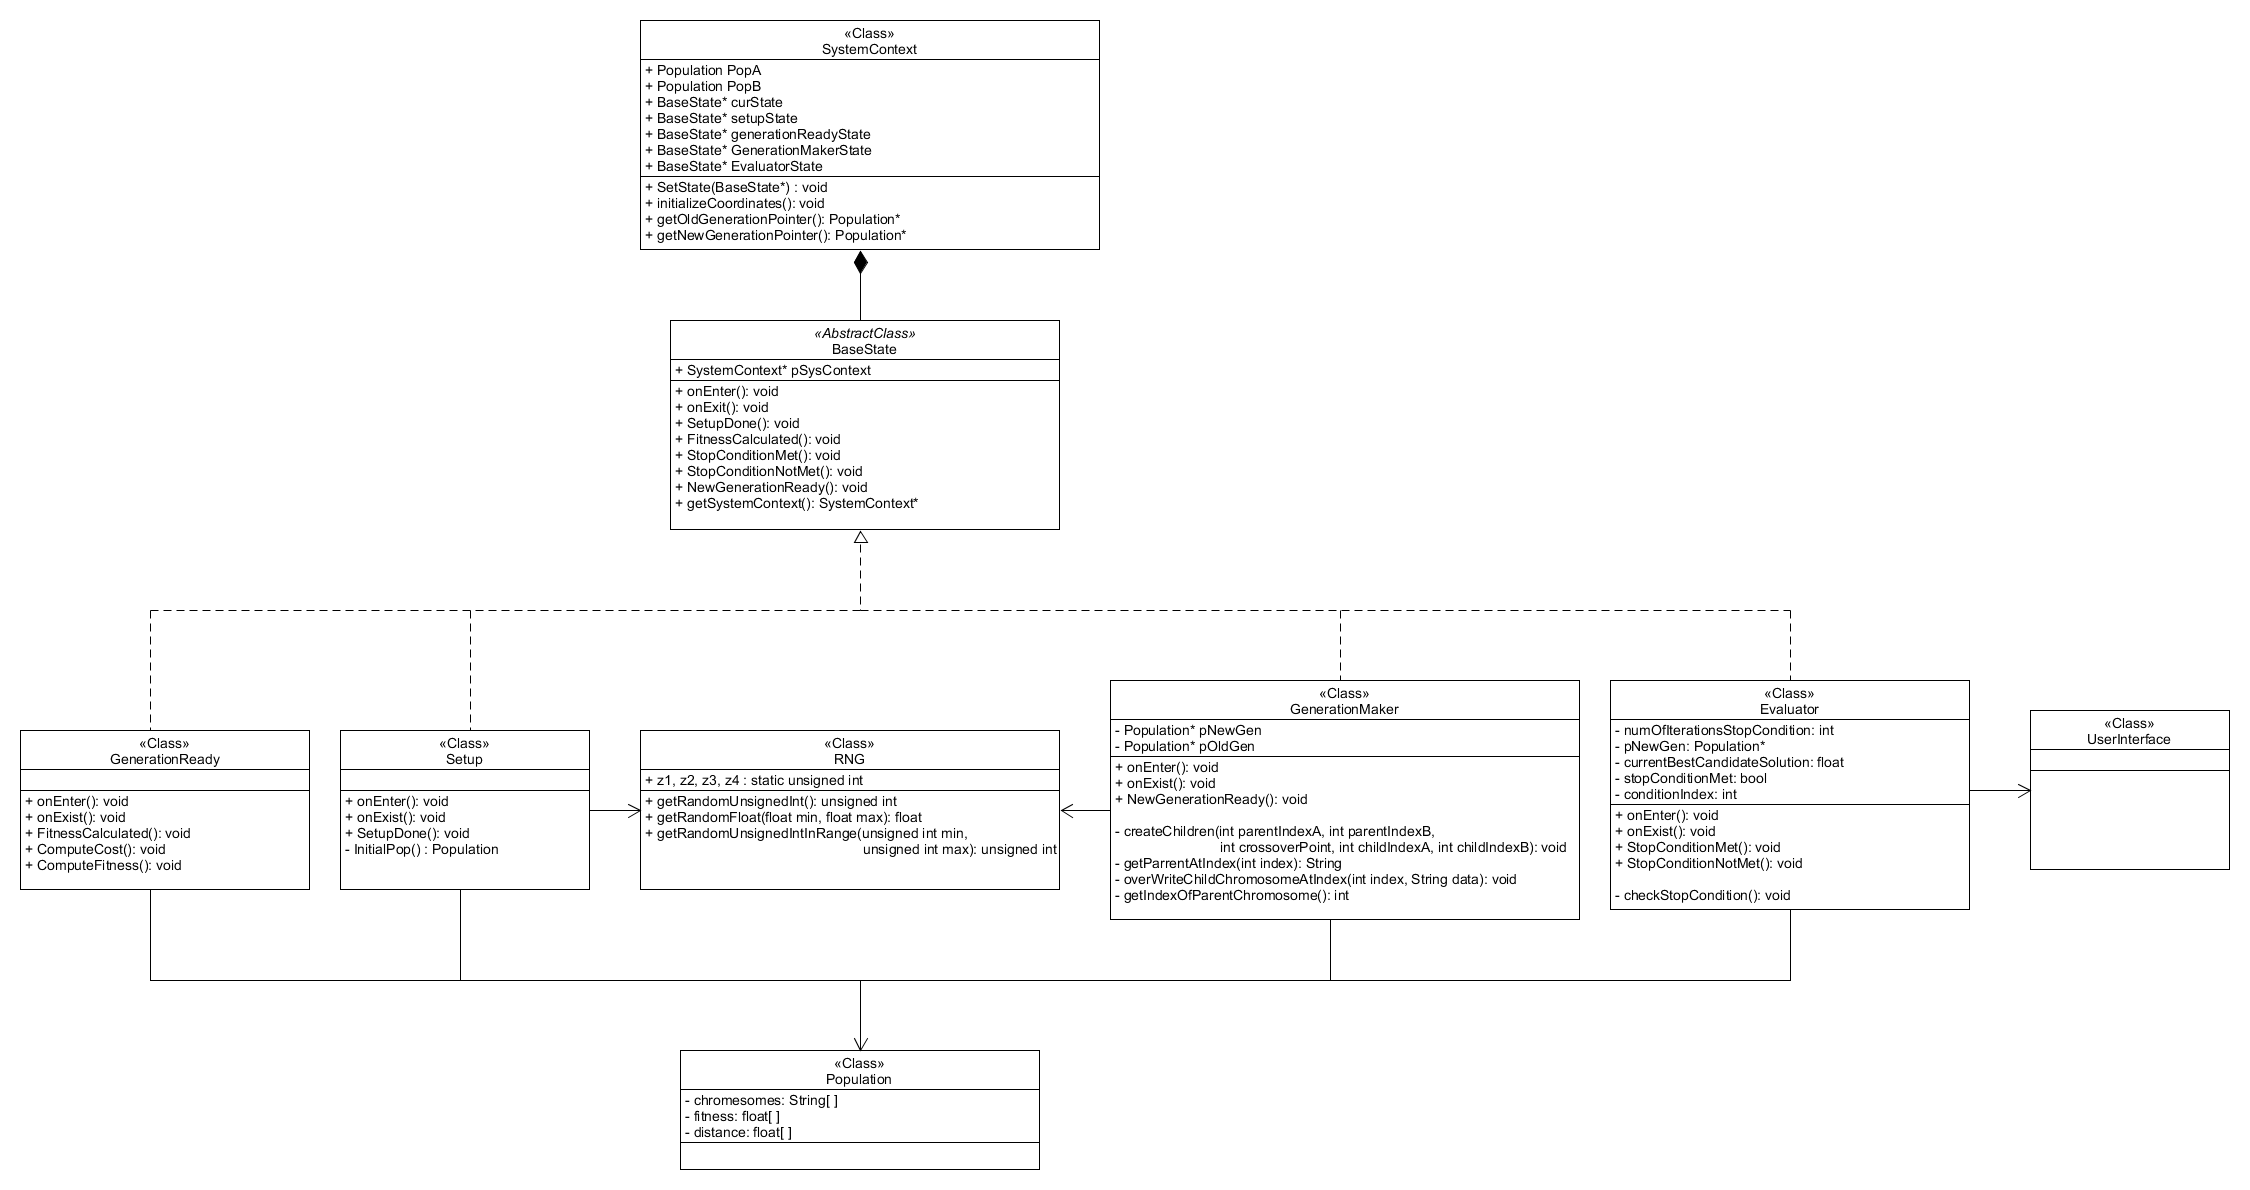
\includegraphics[width=\textwidth]{Images/ClassDiagram.PNG}}\\[0.5cm]
	\caption{Class diagram for the developed system.}
	\label{fig:ClassDiagram}
\end{figure}

As mentioned in the Design chapter a State Machine pattern has been chosen as a good fit for this system and a \textbf{SystemContext} class been created to hold the different states. 